\section{Rounding errors in OWNS-R}~\label{app:Rounding}

In theory, the OWNS-R error decreases with increasing $N_\beta$ if both $\|F_{++}\|$ and $\|F_{--}^{-1}\|$ decrease. However, as discussed in Remark~\ref{rmk:rounding}, computing $\beta_j^*$ numerically (e.g., via \texttt{roots} in MATLAB) introduces rounding errors that prevent convergence. To estimate this rounding error for the 3D oblique-wave breakdown of low-speed Blasius boundary-layer flow in Section~\ref{sec:greedySingle}, we choose random complex numbers $c_k = a_k+ib_k$ with $a_k,b_k\in[-1,1]$ for $k=1,\dots,100$ and compute the relative error in the polynomial approximation as
\begin{equation}
    \max_{k=1,\dots,100}
    \frac{
    |2\prod_{j=1}^{N_\beta}(c_k-\beta_*^j)
    -\prod_{j=1}^{N_\beta}(c_k-\beta_-^j)
    -\prod_{j=1}^{N_\beta}(c_k-\beta_+^j)|}
    {|\prod_{j=1}^{N_\beta}(c_k-\beta_-^j)
    -\prod_{j=1}^{N_\beta}(c_k-\beta_+^j)|}.
\end{equation}
Figure~\ref{fig:poly_err} shows that this error is an increasing function of $N_\beta$, and future work should investigate how to minimize the impact of this rounding error on OWNS-R.
\begin{figure}
    \centering
    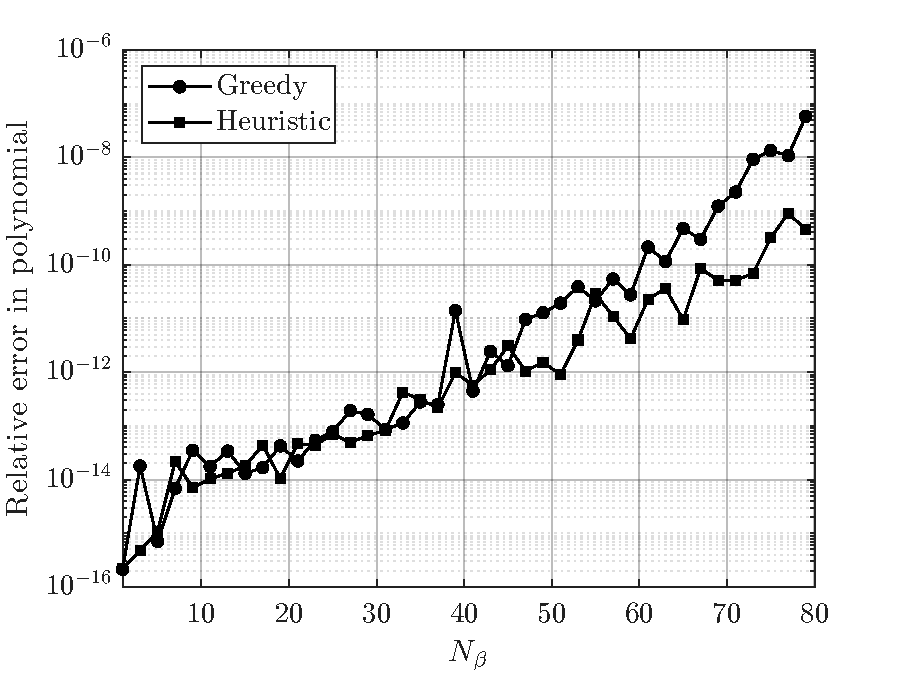
\includegraphics[width=0.5\linewidth]{figures/Oblique_Poly_Err_bw.pdf}
    \caption{The rounding error associated with computing $\beta_*^j$ for OWNS-R increases with increasing $N_\beta$. Demonstration for 3D oblique-wave breakdown of low-speed Blasius boundary-layer flow.}
    \label{fig:poly_err}
\end{figure}